% Options for packages loaded elsewhere
\PassOptionsToPackage{unicode}{hyperref}
\PassOptionsToPackage{hyphens}{url}
%
\documentclass[
]{article}
\usepackage{amsmath,amssymb}
\usepackage{lmodern}
\usepackage{ifxetex,ifluatex}
\ifnum 0\ifxetex 1\fi\ifluatex 1\fi=0 % if pdftex
  \usepackage[T1]{fontenc}
  \usepackage[utf8]{inputenc}
  \usepackage{textcomp} % provide euro and other symbols
\else % if luatex or xetex
  \usepackage{unicode-math}
  \defaultfontfeatures{Scale=MatchLowercase}
  \defaultfontfeatures[\rmfamily]{Ligatures=TeX,Scale=1}
\fi
% Use upquote if available, for straight quotes in verbatim environments
\IfFileExists{upquote.sty}{\usepackage{upquote}}{}
\IfFileExists{microtype.sty}{% use microtype if available
  \usepackage[]{microtype}
  \UseMicrotypeSet[protrusion]{basicmath} % disable protrusion for tt fonts
}{}
\makeatletter
\@ifundefined{KOMAClassName}{% if non-KOMA class
  \IfFileExists{parskip.sty}{%
    \usepackage{parskip}
  }{% else
    \setlength{\parindent}{0pt}
    \setlength{\parskip}{6pt plus 2pt minus 1pt}}
}{% if KOMA class
  \KOMAoptions{parskip=half}}
\makeatother
\usepackage{xcolor}
\IfFileExists{xurl.sty}{\usepackage{xurl}}{} % add URL line breaks if available
\IfFileExists{bookmark.sty}{\usepackage{bookmark}}{\usepackage{hyperref}}
\hypersetup{
  pdftitle={R Notebook template DS at HVL},
  hidelinks,
  pdfcreator={LaTeX via pandoc}}
\urlstyle{same} % disable monospaced font for URLs
\usepackage[margin=1in]{geometry}
\usepackage{color}
\usepackage{fancyvrb}
\newcommand{\VerbBar}{|}
\newcommand{\VERB}{\Verb[commandchars=\\\{\}]}
\DefineVerbatimEnvironment{Highlighting}{Verbatim}{commandchars=\\\{\}}
% Add ',fontsize=\small' for more characters per line
\usepackage{framed}
\definecolor{shadecolor}{RGB}{248,248,248}
\newenvironment{Shaded}{\begin{snugshade}}{\end{snugshade}}
\newcommand{\AlertTok}[1]{\textcolor[rgb]{0.94,0.16,0.16}{#1}}
\newcommand{\AnnotationTok}[1]{\textcolor[rgb]{0.56,0.35,0.01}{\textbf{\textit{#1}}}}
\newcommand{\AttributeTok}[1]{\textcolor[rgb]{0.77,0.63,0.00}{#1}}
\newcommand{\BaseNTok}[1]{\textcolor[rgb]{0.00,0.00,0.81}{#1}}
\newcommand{\BuiltInTok}[1]{#1}
\newcommand{\CharTok}[1]{\textcolor[rgb]{0.31,0.60,0.02}{#1}}
\newcommand{\CommentTok}[1]{\textcolor[rgb]{0.56,0.35,0.01}{\textit{#1}}}
\newcommand{\CommentVarTok}[1]{\textcolor[rgb]{0.56,0.35,0.01}{\textbf{\textit{#1}}}}
\newcommand{\ConstantTok}[1]{\textcolor[rgb]{0.00,0.00,0.00}{#1}}
\newcommand{\ControlFlowTok}[1]{\textcolor[rgb]{0.13,0.29,0.53}{\textbf{#1}}}
\newcommand{\DataTypeTok}[1]{\textcolor[rgb]{0.13,0.29,0.53}{#1}}
\newcommand{\DecValTok}[1]{\textcolor[rgb]{0.00,0.00,0.81}{#1}}
\newcommand{\DocumentationTok}[1]{\textcolor[rgb]{0.56,0.35,0.01}{\textbf{\textit{#1}}}}
\newcommand{\ErrorTok}[1]{\textcolor[rgb]{0.64,0.00,0.00}{\textbf{#1}}}
\newcommand{\ExtensionTok}[1]{#1}
\newcommand{\FloatTok}[1]{\textcolor[rgb]{0.00,0.00,0.81}{#1}}
\newcommand{\FunctionTok}[1]{\textcolor[rgb]{0.00,0.00,0.00}{#1}}
\newcommand{\ImportTok}[1]{#1}
\newcommand{\InformationTok}[1]{\textcolor[rgb]{0.56,0.35,0.01}{\textbf{\textit{#1}}}}
\newcommand{\KeywordTok}[1]{\textcolor[rgb]{0.13,0.29,0.53}{\textbf{#1}}}
\newcommand{\NormalTok}[1]{#1}
\newcommand{\OperatorTok}[1]{\textcolor[rgb]{0.81,0.36,0.00}{\textbf{#1}}}
\newcommand{\OtherTok}[1]{\textcolor[rgb]{0.56,0.35,0.01}{#1}}
\newcommand{\PreprocessorTok}[1]{\textcolor[rgb]{0.56,0.35,0.01}{\textit{#1}}}
\newcommand{\RegionMarkerTok}[1]{#1}
\newcommand{\SpecialCharTok}[1]{\textcolor[rgb]{0.00,0.00,0.00}{#1}}
\newcommand{\SpecialStringTok}[1]{\textcolor[rgb]{0.31,0.60,0.02}{#1}}
\newcommand{\StringTok}[1]{\textcolor[rgb]{0.31,0.60,0.02}{#1}}
\newcommand{\VariableTok}[1]{\textcolor[rgb]{0.00,0.00,0.00}{#1}}
\newcommand{\VerbatimStringTok}[1]{\textcolor[rgb]{0.31,0.60,0.02}{#1}}
\newcommand{\WarningTok}[1]{\textcolor[rgb]{0.56,0.35,0.01}{\textbf{\textit{#1}}}}
\usepackage{longtable,booktabs,array}
\usepackage{calc} % for calculating minipage widths
% Correct order of tables after \paragraph or \subparagraph
\usepackage{etoolbox}
\makeatletter
\patchcmd\longtable{\par}{\if@noskipsec\mbox{}\fi\par}{}{}
\makeatother
% Allow footnotes in longtable head/foot
\IfFileExists{footnotehyper.sty}{\usepackage{footnotehyper}}{\usepackage{footnote}}
\makesavenoteenv{longtable}
\usepackage{graphicx}
\makeatletter
\def\maxwidth{\ifdim\Gin@nat@width>\linewidth\linewidth\else\Gin@nat@width\fi}
\def\maxheight{\ifdim\Gin@nat@height>\textheight\textheight\else\Gin@nat@height\fi}
\makeatother
% Scale images if necessary, so that they will not overflow the page
% margins by default, and it is still possible to overwrite the defaults
% using explicit options in \includegraphics[width, height, ...]{}
\setkeys{Gin}{width=\maxwidth,height=\maxheight,keepaspectratio}
% Set default figure placement to htbp
\makeatletter
\def\fps@figure{htbp}
\makeatother
\usepackage[normalem]{ulem}
% Avoid problems with \sout in headers with hyperref
\pdfstringdefDisableCommands{\renewcommand{\sout}{}}
\setlength{\emergencystretch}{3em} % prevent overfull lines
\providecommand{\tightlist}{%
  \setlength{\itemsep}{0pt}\setlength{\parskip}{0pt}}
\setcounter{secnumdepth}{-\maxdimen} % remove section numbering
\usepackage{amsmath} \usepackage{mathtools}
\ifluatex
  \usepackage{selnolig}  % disable illegal ligatures
\fi
\newlength{\cslhangindent}
\setlength{\cslhangindent}{1.5em}
\newlength{\csllabelwidth}
\setlength{\csllabelwidth}{3em}
\newenvironment{CSLReferences}[2] % #1 hanging-ident, #2 entry spacing
 {% don't indent paragraphs
  \setlength{\parindent}{0pt}
  % turn on hanging indent if param 1 is 1
  \ifodd #1 \everypar{\setlength{\hangindent}{\cslhangindent}}\ignorespaces\fi
  % set entry spacing
  \ifnum #2 > 0
  \setlength{\parskip}{#2\baselineskip}
  \fi
 }%
 {}
\usepackage{calc}
\newcommand{\CSLBlock}[1]{#1\hfill\break}
\newcommand{\CSLLeftMargin}[1]{\parbox[t]{\csllabelwidth}{#1}}
\newcommand{\CSLRightInline}[1]{\parbox[t]{\linewidth - \csllabelwidth}{#1}\break}
\newcommand{\CSLIndent}[1]{\hspace{\cslhangindent}#1}

\title{R Notebook template DS at HVL}
\author{}
\date{\vspace{-2.5em}}

\begin{document}
\maketitle

\begin{verbatim}
---
title: "R Notebook template DS at HVL"
bibliography: ds_course_tmpl.bib
csl: springer-basic-author-date.csl
header-includes:
- \usepackage{amsmath}
- \usepackage{mathtools}
output:
  html_notebook: default
  pdf_document:
    latex_engine: xelatex
    citation_package: natbib
auther: Arnstein Gjestland
fig_caption: true
---
\end{verbatim}

Det en ser ovenfor her er den såkalte YAML headeren til documentet. Den
bestemmer bl.a. hvilket format vi vil ha \texttt{RMarkdown} dokumentet
konvertert til. Her settes også navnet på \texttt{Bibliography}filen vi
vil benytte. Den inneholder vår samling av referanser. Bare de
referansene vi siterer i teksten vil bli lagt til referanselisten.
RStudio vil selv endre litt i YAML, spesielt gjelder dette
\texttt{output:} verdien som blir endret hvis vi velger et annet format
i \texttt{Preview}menyen.

Her tester vi matte \(\bar{x} = \frac{\sum_{i=1}^{N} x_i}{N \cdot y}\)

\[\bar{x} = \frac{\sum_{i=1}^{N} x_i}{N \cdot y}\] \$\$\bar\{x\} =
\frac{1}{N} \sum\_\{i=1\}\^{}\{N\} x\_i

\begin{Shaded}
\begin{Highlighting}[]
\NormalTok{my\_mod }\OtherTok{\textless{}{-}} \FunctionTok{lm}\NormalTok{(dist }\SpecialCharTok{\textasciitilde{}}\NormalTok{ speed, }\AttributeTok{data =}\NormalTok{ cars)}
\FunctionTok{summary}\NormalTok{(my\_mod)}
\end{Highlighting}
\end{Shaded}

\begin{verbatim}
## 
## Call:
## lm(formula = dist ~ speed, data = cars)
## 
## Residuals:
##     Min      1Q  Median      3Q     Max 
## -29.069  -9.525  -2.272   9.215  43.201 
## 
## Coefficients:
##             Estimate Std. Error t value Pr(>|t|)    
## (Intercept) -17.5791     6.7584  -2.601   0.0123 *  
## speed         3.9324     0.4155   9.464 1.49e-12 ***
## ---
## Signif. codes:  0 '***' 0.001 '**' 0.01 '*' 0.05 '.' 0.1 ' ' 1
## 
## Residual standard error: 15.38 on 48 degrees of freedom
## Multiple R-squared:  0.6511, Adjusted R-squared:  0.6438 
## F-statistic: 89.57 on 1 and 48 DF,  p-value: 1.49e-12
\end{verbatim}

\begin{Shaded}
\begin{Highlighting}[]
\FunctionTok{pander}\NormalTok{(my\_mod)}
\end{Highlighting}
\end{Shaded}

\begin{longtable}[]{@{}
  >{\centering\arraybackslash}p{(\columnwidth - 8\tabcolsep) * \real{0.25}}
  >{\centering\arraybackslash}p{(\columnwidth - 8\tabcolsep) * \real{0.15}}
  >{\centering\arraybackslash}p{(\columnwidth - 8\tabcolsep) * \real{0.18}}
  >{\centering\arraybackslash}p{(\columnwidth - 8\tabcolsep) * \real{0.14}}
  >{\centering\arraybackslash}p{(\columnwidth - 8\tabcolsep) * \real{0.15}}@{}}
\caption{Fitting linear model: dist \textasciitilde{}
speed}\tabularnewline
\toprule
~ & Estimate & Std. Error & t value &
Pr(\textgreater\textbar t\textbar) \\
\midrule
\endfirsthead
\toprule
~ & Estimate & Std. Error & t value &
Pr(\textgreater\textbar t\textbar) \\
\midrule
\endhead
\textbf{(Intercept)} & -17.58 & 6.758 & -2.601 & 0.01232 \\
\textbf{speed} & 3.932 & 0.4155 & 9.464 & 1.49e-12 \\
\bottomrule
\end{longtable}

\begin{Shaded}
\begin{Highlighting}[]
\FunctionTok{pander}\NormalTok{(}\FunctionTok{summary}\NormalTok{(my\_mod))}
\end{Highlighting}
\end{Shaded}

\begin{longtable}[]{@{}
  >{\centering\arraybackslash}p{(\columnwidth - 8\tabcolsep) * \real{0.25}}
  >{\centering\arraybackslash}p{(\columnwidth - 8\tabcolsep) * \real{0.15}}
  >{\centering\arraybackslash}p{(\columnwidth - 8\tabcolsep) * \real{0.18}}
  >{\centering\arraybackslash}p{(\columnwidth - 8\tabcolsep) * \real{0.14}}
  >{\centering\arraybackslash}p{(\columnwidth - 8\tabcolsep) * \real{0.15}}@{}}
\toprule
~ & Estimate & Std. Error & t value &
Pr(\textgreater\textbar t\textbar) \\
\midrule
\endhead
\textbf{(Intercept)} & -17.58 & 6.758 & -2.601 & 0.01232 \\
\textbf{speed} & 3.932 & 0.4155 & 9.464 & 1.49e-12 \\
\bottomrule
\end{longtable}

\begin{longtable}[]{@{}
  >{\centering\arraybackslash}p{(\columnwidth - 6\tabcolsep) * \real{0.21}}
  >{\centering\arraybackslash}p{(\columnwidth - 6\tabcolsep) * \real{0.31}}
  >{\centering\arraybackslash}p{(\columnwidth - 6\tabcolsep) * \real{0.12}}
  >{\centering\arraybackslash}p{(\columnwidth - 6\tabcolsep) * \real{0.24}}@{}}
\caption{Fitting linear model: dist \textasciitilde{}
speed}\tabularnewline
\toprule
Observations & Residual Std. Error & \(R^2\) & Adjusted \(R^2\) \\
\midrule
\endfirsthead
\toprule
Observations & Residual Std. Error & \(R^2\) & Adjusted \(R^2\) \\
\midrule
\endhead
50 & 15.38 & 0.6511 & 0.6438 \\
\bottomrule
\end{longtable}

\begin{Shaded}
\begin{Highlighting}[]
\NormalTok{cars[}\DecValTok{1}\SpecialCharTok{:}\DecValTok{10}\NormalTok{,]}
\end{Highlighting}
\end{Shaded}

\begin{verbatim}
##    speed dist
## 1      4    2
## 2      4   10
## 3      7    4
## 4      7   22
## 5      8   16
## 6      9   10
## 7     10   18
## 8     10   26
## 9     10   34
## 10    11   17
\end{verbatim}

\begin{Shaded}
\begin{Highlighting}[]
\FunctionTok{pander}\NormalTok{(cars[}\DecValTok{1}\SpecialCharTok{:}\DecValTok{10}\NormalTok{,])}
\end{Highlighting}
\end{Shaded}

\begin{longtable}[]{@{}
  >{\centering\arraybackslash}p{(\columnwidth - 2\tabcolsep) * \real{0.11}}
  >{\centering\arraybackslash}p{(\columnwidth - 2\tabcolsep) * \real{0.11}}@{}}
\toprule
speed & dist \\
\midrule
\endhead
4 & 2 \\
4 & 10 \\
7 & 4 \\
7 & 22 \\
8 & 16 \\
9 & 10 \\
10 & 18 \\
10 & 26 \\
10 & 34 \\
11 & 17 \\
\bottomrule
\end{longtable}

\begin{Shaded}
\begin{Highlighting}[]
\FunctionTok{pander}\NormalTok{(}\FunctionTok{density}\NormalTok{(}\FunctionTok{runif}\NormalTok{(}\DecValTok{10}\NormalTok{)))}
\end{Highlighting}
\end{Shaded}

\begin{longtable}[]{@{}
  >{\centering\arraybackslash}p{(\columnwidth - 4\tabcolsep) * \real{0.19}}
  >{\centering\arraybackslash}p{(\columnwidth - 4\tabcolsep) * \real{0.19}}
  >{\centering\arraybackslash}p{(\columnwidth - 4\tabcolsep) * \real{0.24}}@{}}
\caption{Kernel density of \emph{runif(10)} (bandwidth:
0.197115)}\tabularnewline
\toprule
~ & Coordinates & Density values \\
\midrule
\endfirsthead
\toprule
~ & Coordinates & Density values \\
\midrule
\endhead
\textbf{Min.} & -0.5666 & 0.003156 \\
\textbf{1st Qu.} & -0.03763 & 0.09851 \\
\textbf{Median} & 0.4914 & 0.5401 \\
\textbf{Mean} & 0.4914 & 0.4719 \\
\textbf{3rd Qu.} & 1.02 & 0.7926 \\
\textbf{Max.} & 1.549 & 0.9079 \\
\bottomrule
\end{longtable}

\begin{Shaded}
\begin{Highlighting}[]
\FunctionTok{chisq.test}\NormalTok{(}\FunctionTok{table}\NormalTok{(mtcars}\SpecialCharTok{$}\NormalTok{am, mtcars}\SpecialCharTok{$}\NormalTok{gear))}
\end{Highlighting}
\end{Shaded}

\begin{verbatim}
## 
##  Pearson's Chi-squared test
## 
## data:  table(mtcars$am, mtcars$gear)
## X-squared = 20.945, df = 2, p-value = 2.831e-05
\end{verbatim}

\begin{Shaded}
\begin{Highlighting}[]
\FunctionTok{pander}\NormalTok{(}\FunctionTok{chisq.test}\NormalTok{(}\FunctionTok{table}\NormalTok{(mtcars}\SpecialCharTok{$}\NormalTok{am, mtcars}\SpecialCharTok{$}\NormalTok{gear)))}
\end{Highlighting}
\end{Shaded}

\begin{longtable}[]{@{}
  >{\centering\arraybackslash}p{(\columnwidth - 4\tabcolsep) * \real{0.24}}
  >{\centering\arraybackslash}p{(\columnwidth - 4\tabcolsep) * \real{0.07}}
  >{\centering\arraybackslash}p{(\columnwidth - 4\tabcolsep) * \real{0.25}}@{}}
\caption{Pearson's Chi-squared test:
\texttt{table(mtcars\$am,\ mtcars\$gear)}}\tabularnewline
\toprule
Test statistic & df & P value \\
\midrule
\endfirsthead
\toprule
Test statistic & df & P value \\
\midrule
\endhead
20.94 & 2 & 2.831e-05 * * * \\
\bottomrule
\end{longtable}

Vi starter med en RMarkdown notebook og vil til slutt konvertere den til
andre formater.

\hypertarget{vivamus-sagittis-lacus-vel-augue-laoreet-rutrum-faucibus.-second-level-header}{%
\subsection{Vivamus sagittis lacus vel augue laoreet rutrum faucibus.
(Second level
header)}\label{vivamus-sagittis-lacus-vel-augue-laoreet-rutrum-faucibus.-second-level-header}}

Plura mihi bona sunt, inclinet, amari petere vellent. Idque Caesaris
facere voluntate liceret: sese habere. Etiam habebis sem dicantur magna
mollis euismod. Quid securi etiam tamquam eu fugiat nulla pariatur.

\hypertarget{formatering-av-tekst}{%
\subsubsection{Formatering av tekst}\label{formatering-av-tekst}}

Overskriften ovenfor er satt vha.
\texttt{\#\#\#\ Formatering\ av\ tekst} på en egen linje (blank linje
før og etter) og er tredje nivå.

\emph{Kursiv} settes vha. \texttt{*Kursiv*} og \textbf{uthevet} skrift
vha. \texttt{**uthevet**}. Hevet tekst får vi vha. \texttt{\^{}} (f.eks.
x\textsuperscript{2} er \texttt{x\^{}2\^{}}), mens senket tekst får vi
ved \texttt{\textasciitilde{}} gjerne kalt «tilde» (f.eks.
y\textsubscript{2} er \texttt{y\textasciitilde{}2\textasciitilde{}}).
Ønsker vi å skrive \texttt{Markdown} kode som \emph{ikke} skal evelures
setter vi den mellom to `, f.eks `\texttt{x\^{}2\^{}}`. Det siste bruker
jeg mye av i dette dokumentet. Ofte er ` en såkalt «dead letter», den er
brukt til å sette merke på bokstaver, så vi trenger en \texttt{space}
etter den siste.

\hypertarget{liste}{%
\paragraph{Liste}\label{liste}}

Overskriften ovenfor er satt vha. \texttt{\#\#\#\#\ Liste} på en egen
linje (blank linje før og etter) og er fjerde nivå.

\hypertarget{uordnete-lister}{%
\subparagraph{Uordnete lister}\label{uordnete-lister}}

Dette er et eksempel på overskrift på femte og laveste nivå. Den er satt
vha. \texttt{\#\#\#\#\#\ Uordnet\ liste\ med\ underliste} på en egen
linje (blank linje før og etter).

Her er «Space»/Mellomrom angitt som «·». Punkter på første nivå i en
liste starter med -Space altså \texttt{-·}, mens andre nivå starter med
\texttt{··*·} (altså SpaceSpace*Space). Tredje nivå starter med
SpaceSpaceSpaceSpace-Space altså \texttt{····-·} osv..

\hypertarget{ordnete-lister}{%
\subparagraph{Ordnete lister}\label{ordnete-lister}}

Ordnete lister starter med tall), feks \texttt{1)} eller \texttt{8}. Vi
trenger ikke holde orden på nummerene, men det første vil være hvor
nummereringen starter.

\hypertarget{eksempel-puxe5-lister}{%
\subparagraph{Eksempel på lister}\label{eksempel-puxe5-lister}}

\begin{itemize}
\item
  Quae vero Fictum, deserunt mollit anim laborum astutumque!
\item
  auctorem tractata ab fiducia dicuntur.

  \begin{itemize}
  \item
    Quisque placerat facilisis
  \item
    egestas cillum

    \begin{itemize}
    \tightlist
    \item
      dolore.
    \end{itemize}
  \end{itemize}
\item
  Tu quoque, Brute,

  \begin{enumerate}
  \def\labelenumi{\arabic{enumi})}
  \tightlist
  \item
    ordnet underliste
  \item
    trenger ikke holde styr på nummer
  \item
    som vi ser
  \item
    men første angir tallet listen begynner på
  \end{enumerate}
\item
  Fili mi, nihil timor populi, nihil!

  \begin{enumerate}
  \def\labelenumi{\arabic{enumi})}
  \setcounter{enumi}{11}
  \tightlist
  \item
    purus
  \item
    sit
  \item
    amet
  \item
    fermentum
  \end{enumerate}
\end{itemize}

Listen ovenfor er satt vha.

\begin{verbatim}
- Quae vero Fictum, deserunt mollit anim laborum astutumque!
- auctorem tractata ab fiducia dicuntur.
  * Quisque placerat facilisis 
  * egestas cillum 
    - dolore.
- Tu quoque, Brute, 
  1) ordnet underliste
  1) trenger ikke holde styr på nummer
  1) som vi ser
  1) men første angir tallet listen begynner på
- Fili mi, nihil timor populi, nihil!
  12) purus 
  12) sit 
  12) amet 
  13) fermentum
\end{verbatim}

\begin{enumerate}
\def\labelenumi{\arabic{enumi})}
\item
  Cras mattis iudicium purus sit amet fermentum.
\item
  Nihil hic munitissimus habendi senatus locus, nihil horum?

  \begin{enumerate}
  \def\labelenumii{\arabic{enumii})}
  \tightlist
  \item
    At nos hinc posthac,
  \item
    sitientis piros Afros.
  \end{enumerate}
\item
  Integer legentibus erat a ante historiarum dapibus.
\item
  Sed haec quis possit intrepidus aestimare tellus.

  \begin{enumerate}
  \def\labelenumii{\arabic{enumii})}
  \setcounter{enumii}{6}
  \tightlist
  \item
    Tityre, tu patulae recubans sub tegmine fagi dolor.
  \item
    Idque Caesaris facere voluntate liceret: sese habere.
  \end{enumerate}
\end{enumerate}

Listen over er satt vha.

\begin{verbatim}
1) Cras mattis iudicium purus sit amet fermentum.
1) Nihil hic munitissimus habendi senatus locus, nihil horum?
    1) At nos hinc posthac,
    2) sitientis piros Afros.
1) Integer legentibus erat a ante historiarum dapibus.
1) Sed haec quis possit intrepidus aestimare tellus.
      7) Tityre, tu patulae recubans sub tegmine fagi dolor.
      7) Idque Caesaris facere voluntate liceret: sese habere.
\end{verbatim}

Når vi vil angi Markdown kode over flere linjer benytter vi ``` på egen
linje før og etter koden. Se i kildekode filen (.Rmd filen) for
eksempler på dette.

\hypertarget{r-code}{%
\paragraph{R code}\label{r-code}}

Vi kan også sette R kode i dokumentet vårt. Da starter vi med ```\{r\}
på egen linje og avslutter med ``` på egen linje. Nedenfor er et
eksempel på litt R kode som er riktig, men med dårlig stil

\texttt{\textasciigrave{}\textasciigrave{}\textasciigrave{}\{r\}\ x=c(10,20,30)\ y=c(0.5,0.3,0.7)\ plot(x,y)}
```

Benytter vi «Styler» (marker koden og velg \texttt{Style\ selection} fra
\texttt{Addins} menyen) kan vi få den tilpasset til \texttt{tidyverse}
stil. Siden vi er i en såkalt «Notebook» må vi trykke på trekanten til
høyre for å se resultatet.

\begin{Shaded}
\begin{Highlighting}[]
\NormalTok{x }\OtherTok{\textless{}{-}} \FunctionTok{c}\NormalTok{(}\DecValTok{10}\NormalTok{, }\DecValTok{20}\NormalTok{, }\DecValTok{30}\NormalTok{)}
\NormalTok{y }\OtherTok{\textless{}{-}} \FunctionTok{c}\NormalTok{(}\FloatTok{0.5}\NormalTok{, }\FloatTok{0.3}\NormalTok{, }\FloatTok{0.7}\NormalTok{)}
\FunctionTok{plot}\NormalTok{(x, y)}
\end{Highlighting}
\end{Shaded}

\includegraphics{ex-notebook_files/figure-latex/unnamed-chunk-3-1.pdf}

\hypertarget{matematikk}{%
\paragraph{Matematikk}\label{matematikk}}

For å skrive matematikk i RMarkdown benytter man LaTeX (Lamport 1986)
som er en makropakke bygget fra TeX (Knuth 1986) for å skrive
strukturerte documenter. Når vi genererer pdf filer fra RMarkdown går vi
også via LaTeX. Vi skriver matematikk i teksten vha. \texttt{\$\ \$},
f.eks. \(r_m = \sum_{i=1}^N w_i \cdot \bar{r}_i\) vha.
\texttt{\$r\_m\ =\ \textbackslash{}sum\_\{i=1\}\^{}N\ w\_i\ \textbackslash{}cdot\ \textbackslash{}bar\{r\}\_i\$}.
Ønsker vi å sette dette som et uttrykk på egen linje benytter vi
\texttt{\$\$\ \$\$} med blank linje før og etter

\[
r_m = \sum_{i=1}^N w_i \cdot \bar{r}_i, \quad
\beta_m = \sum_{i=1}^N w_i \cdot \beta_i
\]

Dette er satt vha. markup koden

\begin{verbatim}
$$
r_m = \sum_{i=1}^N w_i \cdot \bar{r}_i \quad, \beta_m = \sum_{i=1}^N w_i \cdot \beta_i
$$
\end{verbatim}

Ønsker vi likninger over flere linjer kan vi bruke

\begin{verbatim}
\begin{math}
\begin{aligned}
a^2 + b^2 &= c^2 \\ &= 5
\end{aligned}
\end{math}
\end{verbatim}

som gir oss

\begin{math}
\begin{aligned}
a^2 + b^2 &= c^2 \\ &= 5
\end{aligned}
\end{math}

\texttt{\textbackslash{}begin\{aligned\}} kommer fra en ekstra-pakke til
\$\LaTeX \$ kalt \texttt{amsmath} som gir oss muligheter utover standard
\$\LaTeX \$ matte. Vi lastet \texttt{amsmath} i YAML-headeren i starten
av dokumentet.

Vi kan også få til matte over flere linjer vha. standard \$\LaTeX \$.
Nummererte får vi vha. \texttt{eqnarray}. F.eks vil

\begin{verbatim}
\begin{eqnarray}
r_m &=& \sum_{i=1}^N w_i \cdot \bar{r}_i, \\
\beta_m &=& \sum_{i=1}^N w_i \cdot \beta_i
\end{eqnarray}
\end{verbatim}

gi oss

\begin{eqnarray}
r_m &=& \sum_{i=1}^N w_i \cdot \bar{r}_i, \\
\beta_m &=& \sum_{i=1}^N w_i \cdot \beta_i
\end{eqnarray}

Ønsker vi ikke nummerering kan vi benyttet \texttt{eqnarray*} f.eks

\begin{verbatim}
\begin{eqnarray*}
r_m &=& \sum_{i=1}^N w_i \cdot \bar{r}_i, \\
\beta_m &=& \sum_{i=1}^N w_i \cdot \beta_i
\end{eqnarray*}
\end{verbatim}

som gir

\begin{eqnarray*}
r_m &=& \sum_{i=1}^N w_i \cdot \bar{r}_i, \\
\beta_m &=& \sum_{i=1}^N w_i \cdot \beta_i
\end{eqnarray*}

Et tredje alternativ er å benytte \texttt{eqnarray} og så slå av
nummerering på enkelte linjer vha. \texttt{\textbackslash{}nonumber}

\begin{verbatim}
\begin{eqnarray}
r_m &=& \sum_{i=1}^N w_i \cdot \bar{r}_i, \\
\beta_m &=& \sum_{i=1}^N w_i \cdot \beta_i \nonumber
\end{eqnarray}
\end{verbatim}

som gir

\begin{eqnarray}
r_m &=& \sum_{i=1}^N w_i \cdot \bar{r}_i, \\
\beta_m &=& \sum_{i=1}^N w_i \cdot \beta_i \nonumber
\end{eqnarray}

Som vi ser ovenfor benytter vi \texttt{\textbackslash{}\textbackslash{}}
for å angi ny linje (eller riktigere: slutten ppå en linje). Vær veldig
nøye med \texttt{\&} tegnene. Ellers blir det mye krøll.

Her er et eksempel \sout{sjålet} lånt fra
\href{https://en.wikibooks.org/wiki/LaTeX/Mathematics\#cite_note-amsmath-3}{Wikibooks
LaTeX/Mathematics} som er et greit sted for å finne mer om å skrive
matematikk vha. \$\LaTeX \$. Det siste eksemplet benytter også
\texttt{amsmath} (\texttt{\textbackslash{}cfrac} er definert der) som
gir oss flere muligheter.

\[
x = a_0 + \cfrac{1}{a_1 
          + \cfrac{1}{a_2 
          + \cfrac{1}{a_3 + \cfrac{1}{a_4} } } }
\]

\hypertarget{siteringreferanser}{%
\paragraph{Sitering/referanser}\label{siteringreferanser}}

Siteringer skjer i markdown vha. \texttt{{[}@citekey{]}}, f.eks.
\texttt{{[}@knuth1986texbook{]}} som jeg brukte for å sitere TeX boken
ovenfor. Citekey bestemmer vi i utgangspunktet selv, event. mha. Zotero,
men det kan være greit å ha et system. Pakken \texttt{citr} vil
installere en Addin i RStudio som gjør det lettere å legge inn
siteringer. Opplysningene som skal i referanselisten hentes inn fra
filen som vi anga oppe i YAML headeren,
\texttt{bibliography:\ ds\_course\_tmpl.bib}. Det er veldig viktig at
denne ligger på øverste nivå, dvs det må ikke være noe «whitespace» før
\texttt{bibliography}. Ellers får vi en «Error»

\begin{figure}
\centering
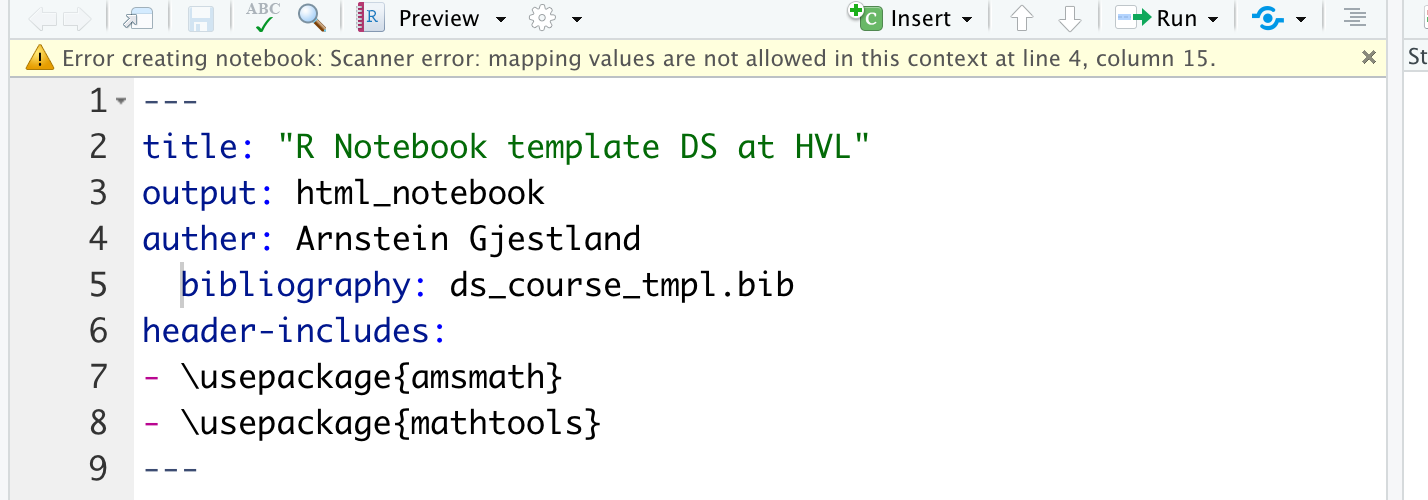
\includegraphics[width=0.7\textwidth,height=\textheight]{bib_error.png}
\caption{Error}
\end{figure}

Informasjon til referanselisten hentes fra bib-filen, her
\texttt{ds\_cource\_tmpl.bib}. For TeX boken er dette

\begin{verbatim}
@book{knuth1986texbook,
  title = {The {{TeXbook}}},
  author = {Knuth, D.E.},
  year = {1986},
  publisher = {{Addison-Wesley}},
  isbn = {978-0-201-13447-6},
  lccn = {85030845},
  series = {Computers \& Typesetting}
}
\end{verbatim}

Dette er ingen fornøyelse å skrive inn selv (tro meg, jeg har gjort det)
så heldigvis har vi nå verktøy som gjør at vi lett kan \sout{stjele}
hente opplysningene fra andre f.eks. Oria (Bibsys) eller andre nettarkiv
(se eget dok. om Zotero).

Systemet fungerer slik at bare det vi referer i teksten blir tatt inn i
referanselisten. Bib-filen kan altså inneholde mange flere kilder en de
vi bruker. Hvordan siteringene ser ut og hvordan referanselisten er
formatert bestemmes av en såkalt \texttt{csl} fil (kan hentes fra
\href{https://www.zotero.org/styles}{Zotero Style Repository}). Denne
legges helst i samme mappe som vårt dokument og må angis i YAML
headeren.

Vi har også tre ulike varianter av cite kommandoen som vi skifter mellom
alt etter hvordan vi siterer. Disse er (Knuth 1986) vha. kommandoen
\texttt{{[}@knuth1986texbook{]}}, (1986) vha. kommandoen
\texttt{{[}-@knuth1986texbook{]}} og Knuth (1986) vha. kommandoen
\texttt{@knuth1986texbook}.

En siste ting er av vi kanskje bør referere til R (R Core Team 2019) og
de fantastiske pakkene vi bruker slik som \texttt{citr} (Aust 2019) etc.
Dette kan vi enklet gjøre ved å benytte R fuksjonen \texttt{citation()}
i \texttt{Console}.

\begin{figure}
\centering
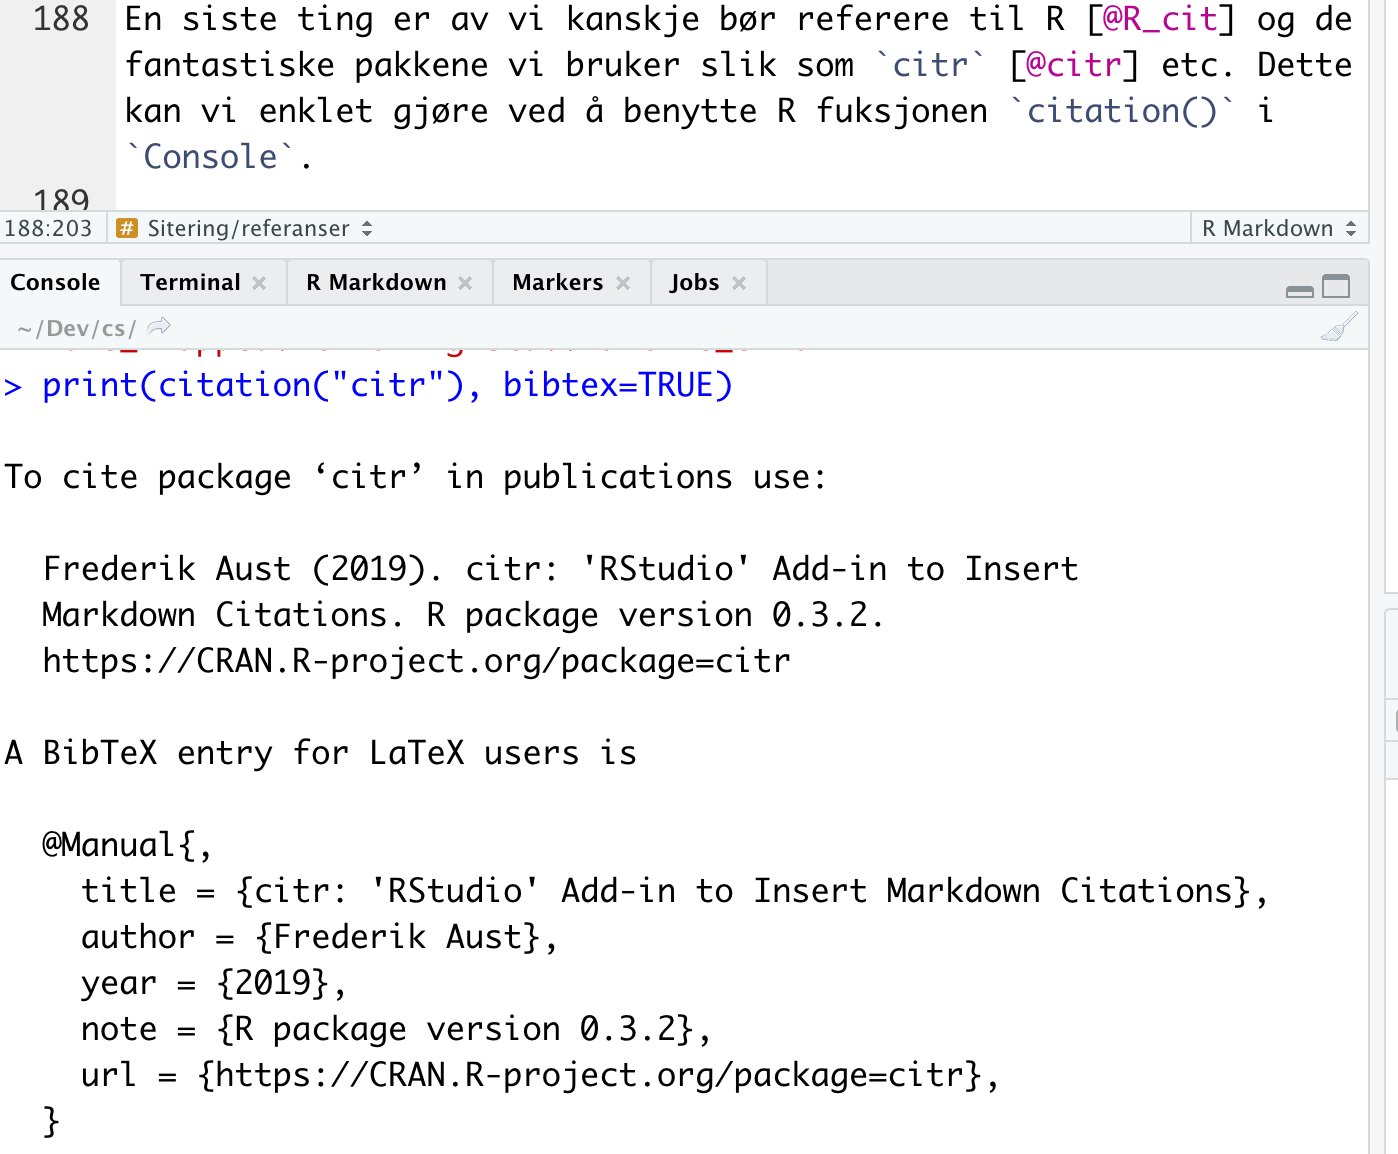
\includegraphics[width=0.7\textwidth,height=\textheight]{cit_citr.png}
\caption{``citr cite''}
\end{figure}

\emph{Fig. 1: Bruk av \texttt{citation()} funksjonen in Console.
\texttt{@Manual\{\}} etc. må kopieres inn i bib-filen. I \texttt{citr}
må en så klikke på det tomme området under tabellen for å få mulighet
til å lese in den oppdaterte bib-filen.}

Merk at RMarkdown ikke har direkte støtte for å sette en forklaring
(«caption») på figurene. Se gjerne .Rmd filen for å se hvordan jeg har
trikset det til her.

Etter å ha gjort tilsvarende for \texttt{knitr} (Xie 2014) (husk å legge
inn cite-key før første komma i bib-filen. Jeg valgte å bruke
\texttt{cit\_knitr}.).

\begin{verbatim}
@InCollection{cit_knitr,
    booktitle = {Implementing Reproducible Computational Research},
    editor = {Victoria Stodden and Friedrich Leisch and Roger D. Peng},
    title = {kn
\end{verbatim}

Jeg har også benyttet pakkene \texttt{RMarkdown} (Xie et al. 2018) og
\texttt{styler} (Müller and Walthert 2020).

Foreløpig har vi bare generert html-dokumenter, men mye av poenget med
\texttt{RMarkdown} er at vi lett skal kunne generere dokumentet i ulike
format. Bruk Knit/Preview menyen og generer pdf og MS Word versjoner.

\hypertarget{referanser}{%
\section*{Referanser}\label{referanser}}
\addcontentsline{toc}{section}{Referanser}

\hypertarget{refs}{}
\begin{CSLReferences}{1}{0}
\leavevmode\hypertarget{ref-citr}{}%
Aust F (2019) Citr: 'RStudio' add-in to insert markdown citations

\leavevmode\hypertarget{ref-knuth1986texbook}{}%
Knuth DE (1986) The {TeXbook}. {Addison-Wesley}

\leavevmode\hypertarget{ref-lamport1986}{}%
Lamport L (1986) {LATEX}: A document preparation system.
{Addison-Wesley}, {Reading, Mass}

\leavevmode\hypertarget{ref-cit_styler}{}%
Müller K, Walthert L (2020) Styler: Non-invasive pretty printing of r
code

\leavevmode\hypertarget{ref-R_cit}{}%
R Core Team (2019) R: A language and environment for statistical
computing. R Foundation for Statistical Computing, Vienna, Austria

\leavevmode\hypertarget{ref-cit_knitr}{}%
Xie Y (2014) Knitr: A comprehensive tool for reproducible research in
{R}. In: Stodden V, Leisch F, Peng RD (eds) Implementing reproducible
computational research. Chapman; Hall/CRC

\leavevmode\hypertarget{ref-cit_rmarkdown}{}%
Xie Y, Allaire JJ, Grolemund G (2018) R markdown: The definitive guide.
Chapman; Hall/CRC, Boca Raton, Florida

\end{CSLReferences}

\end{document}
